\chapter{Background and Related Work}\label{relatedWork}

%CRN backgrounds, motivation
Traditional analog model for spectrum management resulted into the inefficient utilization of most radio frequency spectrum~\cite{valenta2010survey}. While several mobile network spectrum bands are highly congested, other spectrum bands like TV space and non-commercial radio bands are overly under-utilized. Moreover, these utilization varies depending on time and place resulting into spectrum hole~\cite{tandra2009spectrum}. Subsequently, the notion of cognitive radio was proposed to exploit these temporal and spatial spectrum holes.

%CR definition
\section{Cognitive Radio}
Cognitive radio is a special kind of radio with two unique attributes, cognitive capability and reconfigurability~\cite{akyildiz2006next, thomas2005cognitive, haykin2005cognitive}. Cognitive capability enables cognitive radio to sense its radio environment. The radio environment sensing process involves observing the power in various spectrum bands as well as identifying temporal and spatial spectrum holes~\cite{akyildiz2006next}. On the other hand, reconfigurability helps cognitive radio to communicate over various spectrum bands to improve spectrum utilization based on its spectrum awareness~\cite{jondral2005software}.

Based on these two special characteristics, the primary objective of cognitive radio can be best understood from its widely adopted definition~\cite{federal2005notice}:

\begin{quote}
A cognitive radio is a radio or system that senses its operational electromagnetic environment and can dynamically and autonomously adjust its radio operating parameters to modify system operation, such as maximize throughput, mitigate interference, facilitate interoperability, access secondary markets.
\end{quote}

Given the fixed nature of traditional spectrum allocation, the primary challenge of cognitive radio is to exploit spectrum holes in the licensed band while not causing any interruption to the licensed users. Therefore, while using a temporally and/or spatially free spectrum, if the licensed user starts using the corresponding spectrum, the cognitive radio must have the capability to switch to another spectrum or change its other transmission parameters to avoid interruption with the licensed user. Next, we will see how does a cognitive radio achieve this in greater detail.

\subsection{Working Method of A Cognitive Radio}

\begin{figure}[!htbp]
\begin{center}
    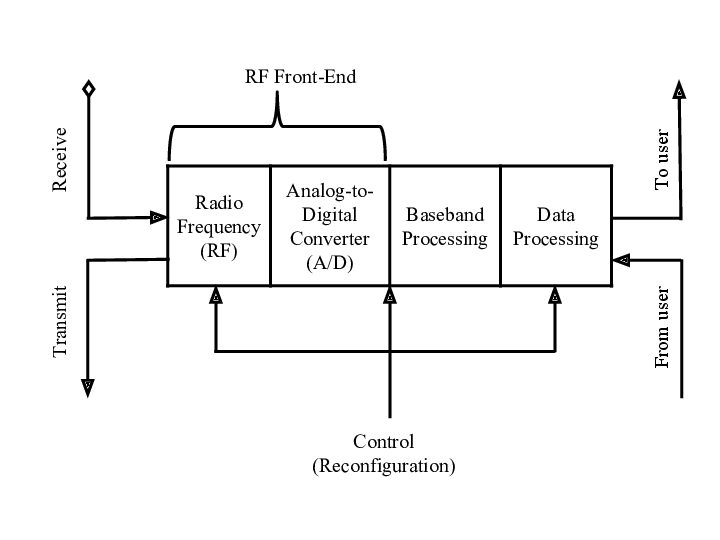
\includegraphics[scale=0.5]{myFigures/PhysicalCR}
    \caption{Cognitive radio transceiver (redrawn from~\cite{jondral2005software})}
    \label{fig:PhysicalCR}
\end{center}
\end{figure}

As shown in Figure~\ref{fig:PhysicalCR}~\cite{jondral2005software}, the cognitive radio transceiver is consisted of a radio front-end and a processing unit~\cite{akyildiz2006next}. The most important fact that distinguishes cognitive radios from other traditional radios is cognitive radio's ability to reconfigure itself via a control bus parameterizing both the radio front-end and processing units~\cite{jondral2005software}. The radio front-end amplifies and mixes the received signal and then converts it from analog to digital signal. The processing unit doing the job of baseband and data processing is quite similar to conventional radio transceivers. Nonetheless, the unique design of cognitive radio's front end also attributes to its novelty, and therefore, we will discuss the radio front-end up next.

\begin{figure}[!htbp]
\begin{center}
    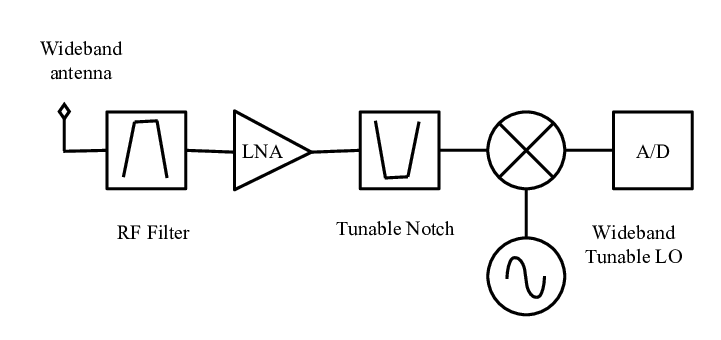
\includegraphics[scale=0.5]{myFigures/RFFrontEnd}
    \caption{Wideband RF/analog front-end architecture for cognitive radio (redrawn from~\cite{cabric2004implementation})}
    \label{fig:RFFrontEnd}
\end{center}
\end{figure}

The radio front-end of a cognitive radio is illustrated in Figure~\ref{fig:RFFrontEnd}~\cite{cabric2004implementation}. It has a wideband sensing capability mainly due to its components like wideband antenna, power amplifier, and adaptive filter. This wideband sensing capability of the radio front end enables cognitive radio to tune to any part of a wide spectrum band. This capability also helps cognitive radio to measure any spectrum information of radio surroundings. To accomplish all this, a wideband radio front-end needs to have several components~\cite{akyildiz2006next}: RF filter, low noise amplifier (LNA), tunable notch, wideband tunable local oscillator (LO), and analog to digital (A/D) converter. RF filter works as a bandpass filter selecting only the desired band RF signal. LNA minimizes the signal noise and amplifies the desired signals amplitude. Tunable notch filters the selected channel from the signal and rejects adjacent channels. Wideband tunable LO has mainly two components: voltage-controlled oscillator (VCO) and mixer. VCO usually can generate signals at any specific frequency and this locally generated RF signal is mixed with desired signal at mixer to convert it into a baseband signal. A/D converter samples and quantizes this signal with very high resolution.

Now that we have described the definition and the working procedure of cognitive radios, we will see how the cognitive radio networks (CRNs) architecture employs cognitive radios to increase spectrum utilization. 

\section{Cognitive Radio Networks (CRNs)}

The Cognitive Radio Networks (CRNs) architecture is shown in Figure~\ref{fig:cogArch}. The components of the architecture can be widely categorized in two groups, the primary network and the secondary network~\cite{akyildiz2006next}. The primary network is the existing network infrastructure. In the existing infrastructure, some spectrum bands are licensed (Example, cellular network, TV broadcast networks) and some other bands are unlicensed. Licensed band users have exclusive right to their spectrum band and are called primary users (PUs). Primary users' access to their licensed band is supervised by the primary base stations and these users require no adaptation to include in cognitive radio networks architecture. 

\begin{figure}[!htbp]
    \begin{center}
        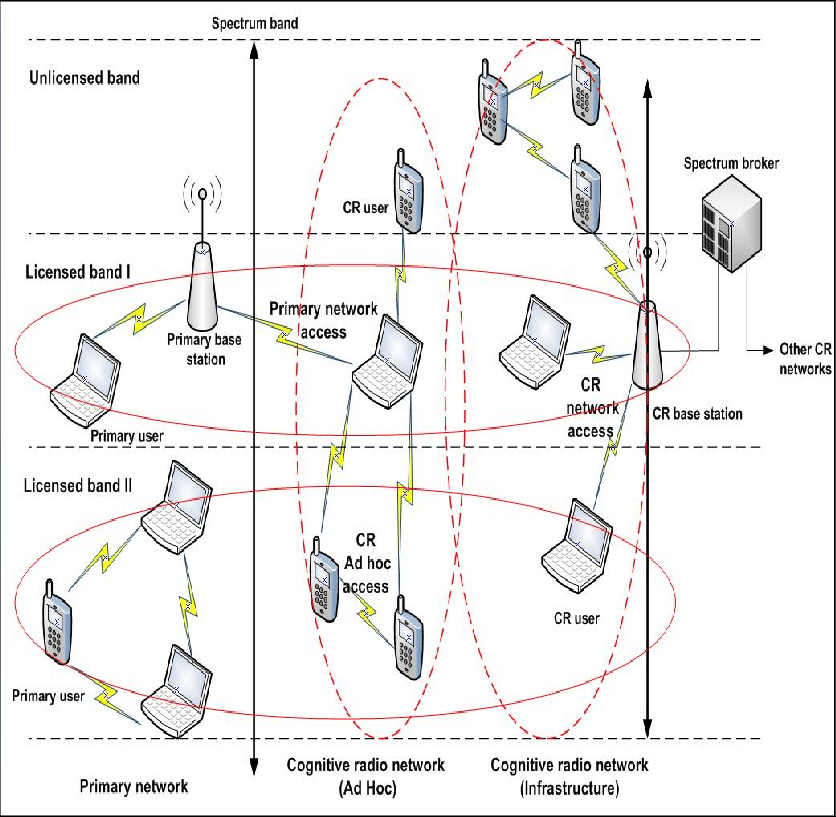
\includegraphics[width=0.6\textwidth]{myFigures/cogArch.png}
        \caption{Cognitive radio networks architecture~\cite{bwnGatechProjectDescription}}
        \label{fig:cogArch}
    \end{center}
\end{figure}

The secondary network is also known as dynamic spectrum access network, unlicensed network, xG network, and cognitive radio network~\cite{akyildiz2006next}. The users of this network contains no license to use the spectrum band and are called secondary users (SUs). These users employ cognitive radios to opportunistically exploit temporal spectrum holes. The secondary network can operate under the provision of secondary base stations or just work in an ad hoc manner. Another important component of cognitive radio networks is a central network entity called spectrum broker that works as a spectrum information manager to maintain the coexistence of multiple cognitive radio networks~\cite{akyildiz2006next, buddhikot2005dimsumnet, ileri2005demand, zekavat2005user}.

\section{Applications of CRNs}
The unconventional architecture of cognitive radio networks has several applications including high-speed rural internet infrastructure development~\cite{fitch2011wireless}, military networks~\cite{murty2003software}, emergency networks~\cite{maldonado2005cognitive}, leased networks~\cite{stine2005spectrum}, and cognitive mesh networks~\cite{berlemann2005policy}.

California based Carlson wireless technologies markets cognitive radio enabled RuralConnect device~\cite{ruralConnect}. This device exploits TV white space to deliver high speed internet connectivity to rural people. It can also be deployed in densly populated areas with significant spectrum contention.

Military networks is another significant applications of CRNs. CRNs support military radios' requirements of choosing any random frequency, modulation and coding techniques, and adaptation to the changing battle-field environment~\cite{akyildiz2006next}.

Emergency networks in the times of natural disasters can be established using CRNs. CRNs establishes such emergency networks by enabling data communication over existing spectrum without installing any new infrastructures~\cite{maldonado2005cognitive}.

\begin{figure}[!htbp]
    \begin{center}
        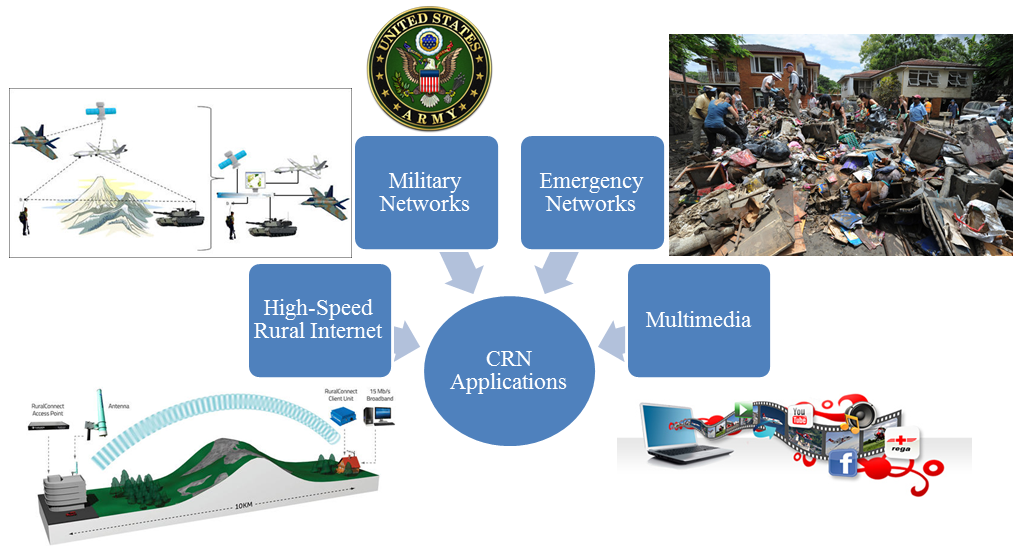
\includegraphics[width=0.8\textwidth]{myFigures/CRNApplications.png}
        \caption{Applications of cognitive radio networks~\cite{akyildiz2006next}}
        \label{fig:CRNApplications}
    \end{center}
\end{figure}

\section{Multi-Radio Networks}

The price of RF transceivers has rapidly reduced in the last few years. This price reduction has prompted to install multiple low-cost radios in a single node of wireless networks~\cite{raniwala2005architecture}. Such networks are known as multi-radio networks. These multi-radio networks impose unique research challenges due to the nature of two conflicting objectives: channel diversity and node connectivity~\cite{wang2007survey}. Multiple radios on a single node enables simultaneous multiple channel access which results in improved network capacity. On the contrary, the transmitter and the receiver must be adjusted to the same channel to maintain network connectivity. Consequently, common control radio based protocols has been proposed in the recent literature to address these challenges~\cite{ko2007distributed, al2016channel, gabale2013classification, kyasanur2006routing, chatterjee2013low}.

One of significant advantage of installing multiple radios on a single node in multi-radio networks is the network performance improvement through parallel spectrum access. On the other hand, the basic motivation behind using cognitive radio networks is also to improve network performance through opportunistic dynamic spectrum access. Therefore, these two paradigms are combined into another network architecture, multi-radio cognitive radio networks. 

\section{Multi-Radio Cognitive Radio Networks(MRCRNs)}
In multi-radio cognitive radio networks, secondary users are equipped with multiple transceivers. This enables secondary users to increase spectrum access just like any multi-radio networks. Moreover, the channel switching time for cognitive radio networks is also reduced as illustrated in Figure~\ref{fig:switchingDelay}. Secondary users have to vacant their currently used channel when the channel's licensed primary user becomes active. This results into secondary users looking for another free channel and switching into that free channel. Secondary users equipped with multiple radios can exploit their additional radios to reduce this switching delay.

\begin{figure}[!htbp]
\begin{center}
    \noindent\begin{minipage}{\textwidth}
    \begin{minipage}[c][6cm][c]{\dimexpr0.5\textwidth-0.5\Colsep\relax}
    \begin{center}
    \begin{tikzpicture} [scale=1.0, transform shape]%show background rectangle,
        \tikzstyle{every node} = [draw, shape = rectangle, node distance=0mm, minimum width=5mm, minimum height=5.2mm]
        \node[draw=black, thick, label=below:Channel 2] (channel2) {
            \begin{tikzpicture}
                \node (puidle) [fill=red!20, minimum width=30mm] {\small Busy};%
            \end{tikzpicture}
        };
        \node[draw=black, thick, label=below:Channel 1] (channel1) [above=of channel2, yshift=7.5mm] {
            
\begin{tikzpicture}
                \node (pubusy) [minimum width=30mm] {\small Idle};
            \end{tikzpicture}
        };
        \node[draw=black, thick, label=below:Channel 3] (channel3) [below=of channel2, yshift=-7.5mm] {
            
\begin{tikzpicture}
                \node (pubusy) [fill=green!20, minimum width=30mm] {\small Idle};
            \end{tikzpicture}
        };
        \node[draw=black, thick, label=below:Channel 4] (channel4) [below=of channel3, yshift=-7.5mm] {
            
\begin{tikzpicture}
                \node (pubusy) [fill=red!20, minimum width=30mm] {\small Busy};
            \end{tikzpicture}
        };

        \node[draw] (mrcrn) [right=of channel3, yshift=0.8cm, xshift=0.25cm] {
            \begin{tikzpicture} [scale=0.625, transform shape]
            \node[draw=white, thick] (su2) [right=of channel3, xshift=1mm] {
            \begin{tikzpicture} [scale=0.5]
            \draw [line width=0.25mm, green!50!black] (2, -0.44) to (2.5,0.44);
            \draw [line width=0.25mm, green!50!black] (3, -0.44) to (2.5,0.44);
            \draw [line width=0.25mm, green!50!black] (2, -0.44) to (3,-0.44);
            \draw [line width=0.25mm, green!50!black] (2.5, -0.44) to (2.5,0.44);
            \draw [fill=green!50!black, green!50!black] (2.5,0.44) circle(1.5mm);

            \draw [line width=0.25mm, green!50!black] (2.5, 0.725) to (2.5,1.0);
            \draw [line width=0.25mm, green!50!black] (2.65, 0.65) to (2.825,0.85);
            \draw [line width=0.25mm, green!50!black] (2.725, 0.44) to (3,0.44);
            \draw [line width=0.25mm, green!50!black] (2.35, 0.65) to (2.175,0.85);
            \draw [line width=0.25mm, green!50!black] (2.275, 0.44) to (2,0.44);

            \end{tikzpicture}
        };

        

        \node[draw=white, thick] (su3) [right=of channel2, xshift=1mm] {
            
\begin{tikzpicture} [scale=0.5]
            \draw [line width=0.25mm] (2, -0.44) to (2.5,0.44);
            \draw [line width=0.25mm] (3, -0.44) to (2.5,0.44);
            \draw [line width=0.25mm] (2, -0.44) to (3,-0.44);
            \draw [line width=0.25mm] (2.5, -0.44) to (2.5,0.44);
            \draw [fill=gray] (2.5,0.44) circle(1.5mm);

            \end{tikzpicture}
        };
        
        \end{tikzpicture}
        };

        \node[draw=white, thick] (pu1) [left=of channel1, xshift=-1mm] {
            
\begin{tikzpicture} [scale=0.5]
            \draw [line width=0.25mm, bend right = 15] (2, -0.44) to (2.5,0.44);
            \draw [line width=0.25mm, bend left = 15] (3, -0.44) to (2.5,0.44);
            \draw [line width=0.25mm] (2.25, -0.15) to (2.75,-0.15);
            %\draw [line width=0.25mm] (2.5, -0.44) to (2.5,0.44);
            \draw [fill=gray] (2.5,0.44) circle(1.5mm);

            \end{tikzpicture}
        };

        \node[draw=white, thick] (pu2) [left=of channel2, xshift=-1mm] {
            
\begin{tikzpicture} [scale=0.5]
            \draw [line width=0.25mm, bend right = 15, red] (2, -0.44) to (2.5,0.44);
            \draw [line width=0.25mm, bend left = 15, red] (3, -0.44) to (2.5,0.44);
            \draw [line width=0.25mm, red] (2.25, -0.15) to (2.75,-0.15);
            %\draw [line width=0.25mm] (2.5, -0.44) to (2.5,0.44);
            \draw [fill=red, red] (2.5,0.44) circle(1.5mm);

            \draw [line width=0.25mm, red] (2.5, 0.725) to (2.5,1.0);
            \draw [line width=0.25mm, red] (2.65, 0.65) to (2.825,0.85);
            \draw [line width=0.25mm, red] (2.725, 0.44) to (3,0.44);
            \draw [line width=0.25mm, red] (2.35, 0.65) to (2.175,0.85);
            \draw [line width=0.25mm, red] (2.275, 0.44) to (2,0.44);

            \end{tikzpicture}
        };

        \node[draw=white, thick] (pu3) [left=of channel3, xshift=-1mm] {
            
\begin{tikzpicture} [scale=0.5]
            \draw [line width=0.25mm, bend right = 15] (2, -0.44) to (2.5,0.44);
            \draw [line width=0.25mm, bend left = 15] (3, -0.44) to (2.5,0.44);
            \draw [line width=0.25mm] (2.25, -0.15) to (2.75,-0.15);
            %\draw [line width=0.25mm] (2.5, -0.44) to (2.5,0.44);
            \draw [fill=gray] (2.5,0.44) circle(1.5mm);

            \end{tikzpicture}
        };

        \node[draw=white, thick] (pu4) [left=of channel4, xshift=-1mm] {
            
\begin{tikzpicture} [scale=0.5]
            \draw [line width=0.25mm, bend right = 15, red] (2, -0.44) to (2.5,0.44);
            \draw [line width=0.25mm, bend left = 15, red] (3, -0.44) to (2.5,0.44);
            \draw [line width=0.25mm, red] (2.25, -0.15) to (2.75,-0.15);
            %\draw [line width=0.25mm] (2.5, -0.44) to (2.5,0.44);
            \draw [fill=red, red] (2.5,0.44) circle(1.5mm);

            \draw [line width=0.25mm, red] (2.5, 0.725) to (2.5,1.0);
            \draw [line width=0.25mm, red] (2.65, 0.65) to (2.825,0.85);
            \draw [line width=0.25mm, red] (2.725, 0.44) to (3,0.44);
            \draw [line width=0.25mm, red] (2.35, 0.65) to (2.175,0.85);
            \draw [line width=0.25mm, red] (2.275, 0.44) to (2,0.44);

            \end{tikzpicture}
        };
    \end{tikzpicture}
    \end{center}
    \end{minipage}\hfill
    \begin{minipage}[c][6cm][c]{\dimexpr0.5\textwidth-0.5\Colsep\relax}
    \begin{center}
    \begin{tikzpicture} [scale=1.0, transform shape]%show background rectangle,
        \tikzstyle{every node} = [draw, shape = rectangle, node distance=0mm, minimum width=5mm, minimum height=5.2mm]
        \node[draw=black, thick, label=below:Channel 2] (channel2) {
            \begin{tikzpicture}
                \node (puidle) [fill=green!20, minimum width=30mm] {\small Idle};%
            \end{tikzpicture}
        };
        \node[draw=black, thick, label=below:Channel 1] (channel1) [above=of channel2, yshift=7.5mm] {
            
\begin{tikzpicture}
                \node (pubusy) [minimum width=30mm] {\small Idle};
            \end{tikzpicture}
        };
        \node[draw=black, thick, label=below:Channel 3] (channel3) [below=of channel2, yshift=-7.5mm] {
            
\begin{tikzpicture}
                \node (pubusy) [fill=red!20, minimum width=30mm] {\small Busy};
            \end{tikzpicture}
        };
        \node[draw=black, thick, label=below:Channel 4] (channel4) [below=of channel3, yshift=-7.5mm] {
            
\begin{tikzpicture}
                \node (pubusy) [fill=red!20, minimum width=30mm] {\small Busy};
            \end{tikzpicture}
        };

        \node[draw] (mrcrn) [right=of channel3, yshift=0.8cm, xshift=0.25cm] {
            \begin{tikzpicture} [scale=0.625, transform shape]

        

        \node[draw=white, thick] (su2) [right=of channel3, xshift=1mm] {
            \begin{tikzpicture} [scale=0.5]
            \draw [line width=0.25mm] (2, -0.44) to (2.5,0.44);
            \draw [line width=0.25mm] (3, -0.44) to (2.5,0.44);
            \draw [line width=0.25mm] (2, -0.44) to (3,-0.44);
            \draw [line width=0.25mm] (2.5, -0.44) to (2.5,0.44);
            \draw [fill=gray] (2.5,0.44) circle(1.5mm);

            \end{tikzpicture}
        };

        \node[draw=white, thick] (su3) [right=of channel2, xshift=1mm] {
            
\begin{tikzpicture} [scale=0.5]
            \draw [line width=0.25mm, green!50!black] (2, -0.44) to (2.5,0.44);
            \draw [line width=0.25mm, green!50!black] (3, -0.44) to (2.5,0.44);
            \draw [line width=0.25mm, green!50!black] (2, -0.44) to (3,-0.44);
            \draw [line width=0.25mm, green!50!black] (2.5, -0.44) to (2.5,0.44);
            \draw [fill=green!50!black, green!50!black] (2.5,0.44) circle(1.5mm);

            \draw [line width=0.25mm, green!50!black] (2.5, 0.725) to (2.5,1.0);
            \draw [line width=0.25mm, green!50!black] (2.65, 0.65) to (2.825,0.85);
            \draw [line width=0.25mm, green!50!black] (2.725, 0.44) to (3,0.44);
            \draw [line width=0.25mm, green!50!black] (2.35, 0.65) to (2.175,0.85);
            \draw [line width=0.25mm, green!50!black] (2.275, 0.44) to (2,0.44);

            \end{tikzpicture}
        };
        \end{tikzpicture}
        };

        \node[draw=white, thick] (pu1) [left=of channel1, xshift=-1mm] {
            
\begin{tikzpicture} [scale=0.5]
            \draw [line width=0.25mm, bend right = 15] (2, -0.44) to (2.5,0.44);
            \draw [line width=0.25mm, bend left = 15] (3, -0.44) to (2.5,0.44);
            \draw [line width=0.25mm] (2.25, -0.15) to (2.75,-0.15);
            %\draw [line width=0.25mm] (2.5, -0.44) to (2.5,0.44);
            \draw [fill=gray] (2.5,0.44) circle(1.5mm);

            \end{tikzpicture}
        };

        \node[draw=white, thick] (pu2) [left=of channel2, xshift=-1mm] {
            
\begin{tikzpicture} [scale=0.5]
            \draw [line width=0.25mm, bend right = 15] (2, -0.44) to (2.5,0.44);
            \draw [line width=0.25mm, bend left = 15] (3, -0.44) to (2.5,0.44);
            \draw [line width=0.25mm] (2.25, -0.15) to (2.75,-0.15);
            %\draw [line width=0.25mm] (2.5, -0.44) to (2.5,0.44);
            \draw [fill=gray] (2.5,0.44) circle(1.5mm);

            \end{tikzpicture}
        };

        \node[draw=white, thick] (pu3) [left=of channel3, xshift=-1mm] {
            
\begin{tikzpicture} [scale=0.5]
            \draw [line width=0.25mm, bend right = 15, red] (2, -0.44) to (2.5,0.44);
            \draw [line width=0.25mm, bend left = 15, red] (3, -0.44) to (2.5,0.44);
            \draw [line width=0.25mm, red] (2.25, -0.15) to (2.75,-0.15);
            %\draw [line width=0.25mm] (2.5, -0.44) to (2.5,0.44);
            \draw [fill=red, red] (2.5,0.44) circle(1.5mm);

            \draw [line width=0.25mm, red] (2.5, 0.725) to (2.5,1.0);
            \draw [line width=0.25mm, red] (2.65, 0.65) to (2.825,0.85);
            \draw [line width=0.25mm, red] (2.725, 0.44) to (3,0.44);
            \draw [line width=0.25mm, red] (2.35, 0.65) to (2.175,0.85);
            \draw [line width=0.25mm, red] (2.275, 0.44) to (2,0.44);

            \end{tikzpicture}
        };

        \node[draw=white, thick] (pu4) [left=of channel4, xshift=-1mm] {
            
\begin{tikzpicture} [scale=0.5]
            \draw [line width=0.25mm, bend right = 15, red] (2, -0.44) to (2.5,0.44);
            \draw [line width=0.25mm, bend left = 15, red] (3, -0.44) to (2.5,0.44);
            \draw [line width=0.25mm, red] (2.25, -0.15) to (2.75,-0.15);
            %\draw [line width=0.25mm] (2.5, -0.44) to (2.5,0.44);
            \draw [fill=red, red] (2.5,0.44) circle(1.5mm);

            \draw [line width=0.25mm, red] (2.5, 0.725) to (2.5,1.0);
            \draw [line width=0.25mm, red] (2.65, 0.65) to (2.825,0.85);
            \draw [line width=0.25mm, red] (2.725, 0.44) to (3,0.44);
            \draw [line width=0.25mm, red] (2.35, 0.65) to (2.175,0.85);
            \draw [line width=0.25mm, red] (2.275, 0.44) to (2,0.44);

            \end{tikzpicture}
        };
    \end{tikzpicture}
    \end{center}
    \end{minipage}%
\end{minipage}

    \caption{Secondary users (SUs) equipped with multiple radios experience reduced switching delay}
    \label{fig:switchingDelay}
\end{center}
\end{figure}

Due to these advantages, several studies have investigated the various research problems in MRCRNs. In next section, we will survey the existing research works on MRCRNs.

\section{Existing Studies on MRCRNs}
Existing studies on MRCRNs mainly investigate how to incorporate multiple radios in dynamic spectrum sharing scenario. These studies mainly propose medium access control protocols~\cite{cormio2009survey, de2012survey}, routing protocols~\cite{zhu2008stod, feng2009joint}, and channel assignment~\cite{ahmadi2012distributed, zhong2014capacity} for MRCRNs. Zhu et al., present a spectrum-tree based on-demand routing protocol that considers multi-radio nodes~\cite{zhu2008stod}. Such nodes belong to multiple spectrum-trees and are called overlapping nodes. As these nodes simultaneously work in different spectrum-trees, they can be used for inter-spectrum routing. The study shows that the proposed approach significantly reduces the average end-to-end delay.  Besides, Feng et al., propose a novel spectrum handoff scheduling approach for multi-hop MRCRNs~\cite{feng2009joint}. This study presents a routing protocol with the help of aging-based priority assignment to minimize the latency. Thus none of these approaches addresses the problem of overcoming throughput degradation problem in MRCRNs.

Ahmadi et al., present one of the earliest CRN studies involving multiple radios, which considers two sender radios for each secondary user~\cite{ahmadi2012distributed}. This study strives to solve channel assignment problem for the scenario. However, as there is only one receiver radio for each user in the proposed network model and channels are assigned to the receiver radio, the corresponding channel assignment problem becomes close to the single-radio channel assignment problem. This is because, as in single-radio scenario, only one channel needs to be assigned for each receiver node and the node can not exploit multiple available channels while receiving packets. Further, the study always uses a fixed number of transmitter radios (two) and do not investigate performance of the network for varying numbers of radios.

Another MRCRN study~\cite{zhong2014capacity} by Zhong et al., aims to solve the channel assignment problem for MRCRNs. Here, their proposed channel assignment approach assigns multiple channels among multiple radios available for secondary users. Despite ranking channels, while assigning them among radios, the approach does not consider the state of those radios. Besides, the paper does not provide any analysis on throughput with an increase in the number of radios.

The analysis of any performance metric based on an increase in the number of radios in CRNs is first presented in the study~\cite{li2014deterministic} by Li et al., to the best of our knowledge. The study presents a rendezvous channel establishment approach for MRCRNs. It shows that the maximum time to rendezvous reduces with an increase in the number of radios used in CRNs. However, the study does not provide any solution on how these radios will be used for data transmission and its subsequent effect on performance metrics such as throughput and delay.

Later, Khan et al.,~\cite{khan2015towards} propose another MRCRNs architecture where each secondary user employs multiple radios for data transmission. The study shows that per packet average end-to-end delay gets improved at the cost of throughput degradation with an increase in the number of radios. This study does the radio-channel assignment in a random manner and does not avoid inter-user channel interface. Thus, this study fails to improve throughput with an increase in the number of radios.

In summary, none of the existing studies focuses on enhancing throughput in MRCRNs. Therefore, we attempt to propose a new channel assignment approach to enhance throughput in MRCRNs in this thesis. Before presenting the approach, we first elaborate our system model and problem formulation.
\endinput
